\documentclass{minimal}
\usepackage{bm}
\usepackage{epsfig,color}
\usepackage[papersize={576.00bp,432.00bp},text={576.00bp,432.00bp}]{geometry}
\begin{document}
\centering
% Title: glps_renderer figure
% Creator: GL2PS 1.3.8, (C) 1999-2012 C. Geuzaine
% For: Octave
% CreationDate: Thu Aug 27 16:54:06 2015
\setlength{\unitlength}{1pt}
\begin{picture}(0,0)
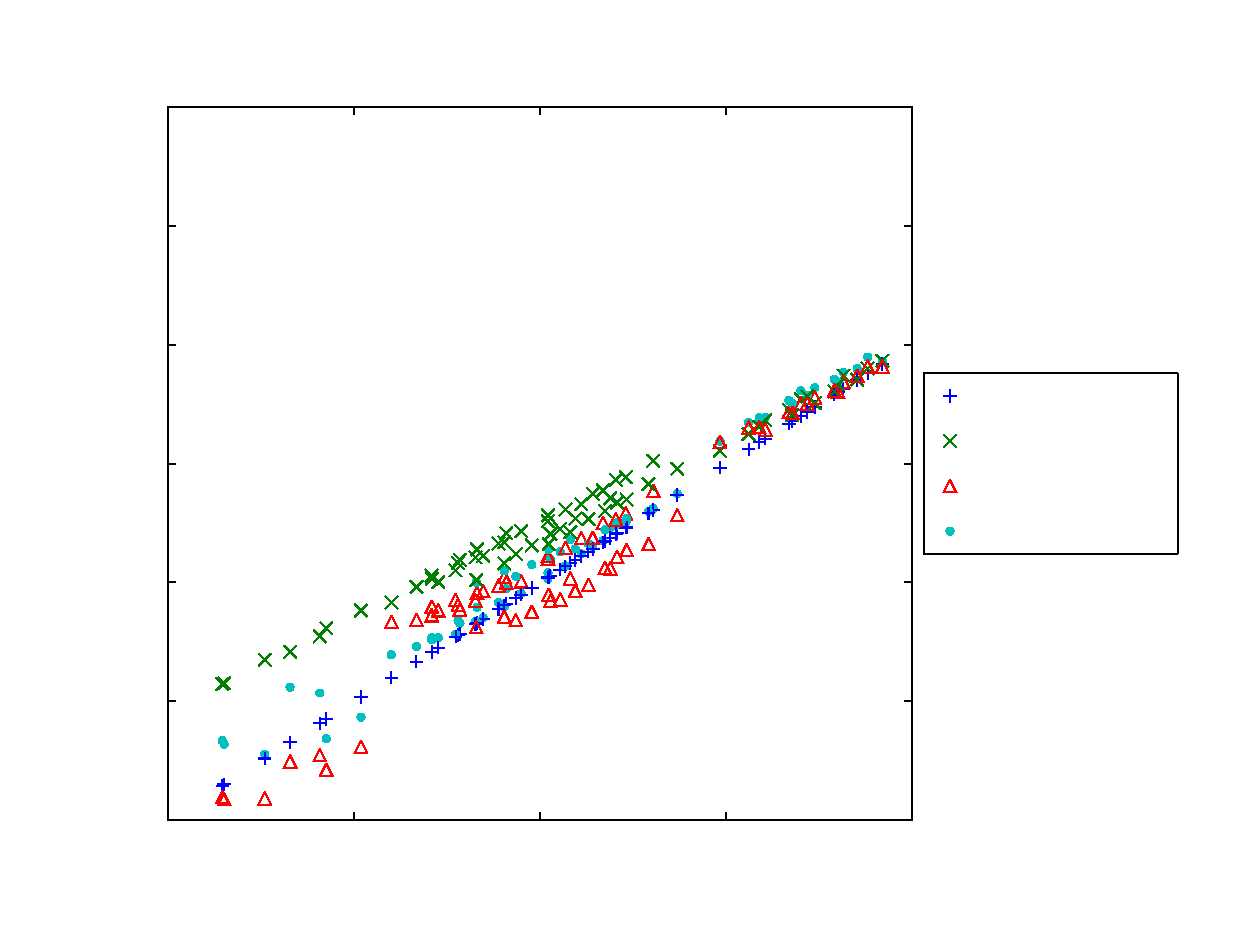
\includegraphics{gs_ab_lm-inc}
\end{picture}%
\begin{picture}(576,432)(0,0)
\fontsize{16}{0}
\selectfont\put(72.7998,41.1958){\makebox(0,0)[t]{\textcolor[rgb]{0,0,0}{{-4}}}}
\fontsize{16}{0}
\selectfont\put(162.09,41.1958){\makebox(0,0)[t]{\textcolor[rgb]{0,0,0}{{-3}}}}
\fontsize{16}{0}
\selectfont\put(251.381,41.1958){\makebox(0,0)[t]{\textcolor[rgb]{0,0,0}{{-2}}}}
\fontsize{16}{0}
\selectfont\put(340.671,41.1958){\makebox(0,0)[t]{\textcolor[rgb]{0,0,0}{{-1}}}}
\fontsize{16}{0}
\selectfont\put(429.961,41.1958){\makebox(0,0)[t]{\textcolor[rgb]{0,0,0}{{0}}}}
\fontsize{16}{0}
\selectfont\put(67.7979,46.2002){\makebox(0,0)[r]{\textcolor[rgb]{0,0,0}{{-4}}}}
\fontsize{16}{0}
\selectfont\put(67.7979,103.25){\makebox(0,0)[r]{\textcolor[rgb]{0,0,0}{{-3}}}}
\fontsize{16}{0}
\selectfont\put(67.7979,160.3){\makebox(0,0)[r]{\textcolor[rgb]{0,0,0}{{-2}}}}
\fontsize{16}{0}
\selectfont\put(67.7979,217.35){\makebox(0,0)[r]{\textcolor[rgb]{0,0,0}{{-1}}}}
\fontsize{16}{0}
\selectfont\put(67.7979,274.4){\makebox(0,0)[r]{\textcolor[rgb]{0,0,0}{{0}}}}
\fontsize{16}{0}
\selectfont\put(67.7979,331.45){\makebox(0,0)[r]{\textcolor[rgb]{0,0,0}{{1}}}}
\fontsize{16}{0}
\selectfont\put(67.7979,388.5){\makebox(0,0)[r]{\textcolor[rgb]{0,0,0}{{2}}}}
\fontsize{16}{0}
\selectfont\put(251.381,28.1958){\makebox(0,0)[t]{\textcolor[rgb]{0,0,0}{{$\Delta E_{clust}^{FHaims}$ [eV]}}}}
\fontsize{16}{0}
\selectfont\put(53.7979,217.35){\rotatebox{90}{\makebox(0,0)[b]{\textcolor[rgb]{0,0,0}{{$\Delta E_{clust}^{meth}$ [eV]}}}}}
\fontsize{16}{0}
\selectfont\put(460.661,249.854){\makebox(0,0)[l]{\textcolor[rgb]{0,0,0}{{gaussian}}}}
\fontsize{16}{0}
\selectfont\put(460.661,228.185){\makebox(0,0)[l]{\textcolor[rgb]{0,0,0}{{abinit}}}}
\fontsize{16}{0}
\selectfont\put(460.661,206.515){\makebox(0,0)[l]{\textcolor[rgb]{0,0,0}{{Lammps (I)}}}}
\fontsize{16}{0}
\selectfont\put(460.661,184.846){\makebox(0,0)[l]{\textcolor[rgb]{0,0,0}{{Lammps (II)}}}}
\end{picture}
\end{document}
